\section{Aufbau und Durchführung}
\subsection{Apperatekonstanten}
Zunächst werden die Apperatekonstaten bestimmt.
Dazu wird zunächst überprüft, welches der drei Geräte vorliegt und die Gerätenummer abgelesen.
Die dazugehörigen Werte werden vom vorliegenden Material abgelesen.
\subsection{Effektiver Widerstand und Abklingzeit \label{sec:Az}}
Um die Amplitudenabnahme des RLC-Kreises zu bestimmen, wird zunächst die folgende Schaltung aufgebaut:
\begin{figure}[H]
  \centering
  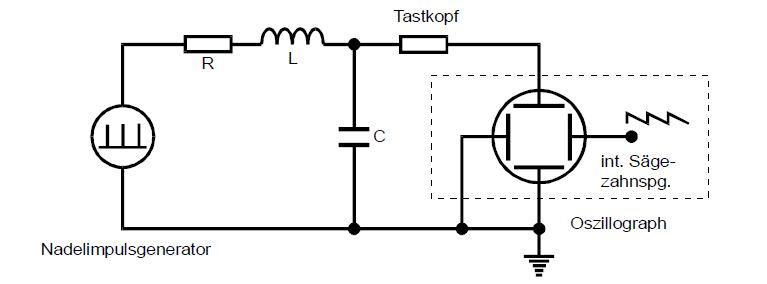
\includegraphics[width=\textwidth]{Text/Nadelimpulsgenerator.jpg}
  \caption{Messschaltung zur Bestimmung des aperiodischen Grenzwiderstandes $R_\text{ap}$ \cite[294]{sample}}
  \label{fig:Aufbau}
\end{figure}
Dabei ist zu beachten, dass der kleinere Widerstand zu verwenden ist.
Sind alle Parameter des Oszilloskops und des Generators optimal eingestellt, so lässt sich nun der Spannungsverlauf
auf dem Bildschirm des Osilloskops erkennen.
Ist dies der Fall, wird der Curser des Oszilloskops auf das lokale Maximum gesetzt
und die Werte der Spannung $U_C$ und der Zeit $t$ abgelesen.
Der Vorgang wird dann 15 mal für andere Maxima wiederholt.
\subsection{Aperiodischer Grenzfall}
Hier wird die gleiche Schaltung wie in \ref{sec:Az} verwendet, mit dem Unterschied, dass
nun ein variabler Widerstand verwendet wird. Dieser wird zunächst auf den kleinsten einstellbaren Widerstand eingestellt.
Danach wird er solange erhöht, bis die Überschwingung der Spannung gerade eben nicht mehr zu beobachten ist.
Der eingestellte Wert wird daraufhin notiert.
\newpage
\subsection{Frequenzabhängigkeit der Spannung\label{FA}}
Um die Frequenzabhängigkeit der Spannung herauszufinden, wird zunächst folgende Schaltung aufgebaut:
\begin{figure}[H]
  \centering
  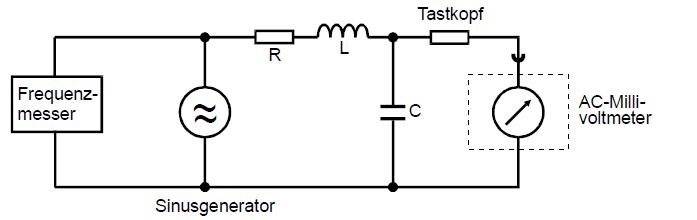
\includegraphics[width=\textwidth]{Text/Frequenzmesser.jpg}
  \caption{Schaltung zur Aufnahme des Frequenzganges eines RLC-Kreises \cite[295]{sample}}
  \label{fig:Aufbau3}
\end{figure}
Die Frequenz am Generator wird möglichst klein eingestellt und an die Schaltung angeschlossen.
Daraufhin sollte bei korrekt eingestelltem Oszillsokop der Spannungsverlauf angezeigt werden.
Ist dies getan, wird die Frequenz am Generator schrittweise erhöht und die jeweilige
Amplitude mit der entsprechenenden Frequenz notiert.
Zu beachten ist dabei jedoch, dass im Bereich $\pm\SI{5}{\kilo\hertz}$ um das ausgerechnete Maximum
die Frequenz in $\SI{1}{\kilo\hertz}$-Schritten erhöht wird.
\subsection{Frequenzabhängigkeit der Phase}
Um die Frequenzabhängig der Phase zwischen Kondensator- und Erregerspannung zu messen, werden beide Spannungen
auf das Oszilloskop abgebildet. Dazu wird folgene Schaltung genutzt:
\begin{figure}[H]
  \centering
  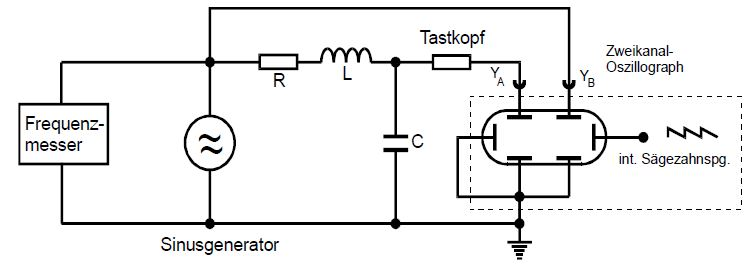
\includegraphics[width=\textwidth]{Text/Frequenzmesser2.jpg}
  \caption{Schaltung zur Messung der Frequenzabhängigkeit der Phase zwischen Erreger- und Kondensatorspannung bei einem RLC-Kreis \cite[296]{sample}}
  \label{fig:Aufbau4}
\end{figure}
Nun wird, wie bei \ref{FA}, die Frequenz eingestellt und daraufhin schrittweise erhöht.
Es werden dieselben Frequenzen verwendet wie in \ref{FA}.
Dabei werden nach jeder Erhöhung die Curser auf die Amplituden der Kurven gelegt. Die Zeitdifferenz $\Delta t$
- in (\ref{fig:Aufbau4})als Abstand $a$ eingetragen - wird daraufhin abgelesen und notiert.
Die Periodenlänge $b$ lässt sich berechnen und muss nicht gemessen werden.
\begin{figure}[H]
  \centering
  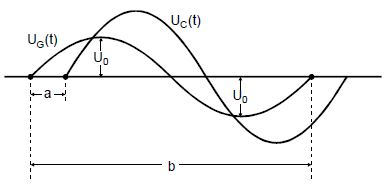
\includegraphics{Text/Kurven.jpg}
  \caption{Phasenverschiebung zweier Spannungen \cite[282]{sample2}}
  \label{fig:Aufbau5}
\end{figure}
